% Chapter 1

\chapter{Test Procedure} % Main chapter title

\label{Chapter1} % For referencing the chapter elsewhere, use \ref{Chapter1} 

%----------------------------------------------------------------------------------------

\section{Introduction}
\section{Electronic test}
For the electronic tests, we test the performance of Optical Follower Servo chassis and Interface chassis using the test procedures from LIGO (DCC number T1400486-v2 and T1400484-v2), but change the expected value to the value we calculated.
\subsection{Optical Follower Servo board test}
\begin{enumerate}
	\item \textbf{Overview}\\
	The PCal Optical Follower Servo Chassis includes two Optical Follower Servo Boards, and two Optical Follower Back Board. The function of this chassis is to drive two AOMs with a whatever voltage is necessary in order to make the light coming out of the AOM match the sinusoidal shape of the excitation signal.
	\item \textbf{Test Equipment}
	\begin{enumerate}
		\item Power Supply capable of ~$\pm$18V,~2A
		\item Digital Multimeter (DMM)
		\item Power Supply
		\item Oscilloscope
		\item Function Generator
		\item Spectrum analyzer
	\end{enumerate}
	
	\item \textbf{DC test}\\
	\begin{enumerate}
		\item Turn on the power supply and the switches, and check the LED status below:
		\begin{center}
			\resizebox{13cm}{!}{
				\begin{tabular}{| c | c | c | c |}
					\hline
					\multirow{2}{*}{\textbf{Voltage}} & \multirow{2}{*}{\textbf{Current}}  & \multirow{2}{*}{\textbf{Observed Current}}  & \textbf{Front Panel LEDs On,}\\
					& & & \textbf{$\pm$15V and $\pm$12V?}\\ \hline
					+18V & 20mA$\pm$ 5mA &   & \\ \hline
					-18V & 19mA$\pm$ 5mA &   & \\
					\hline
				\end{tabular}
			}
		\end{center}
		\item Attach a standard 9-pin breakout board to the D-sub labeled “From PCal PD”. With a DMM, check the voltages on the pins in the table below:
		\begin{center}
			\resizebox{13cm}{!}{
				\begin{tabular}{| c | c | c |}
					\hline
					\textbf{Pins} & \textbf{Voltage Expected} & \textbf{Voltage Observed}\\ \hline
					J1 Pin2(+) and 7(GND) & +15V$\pm$ 0.5V & \\ \hline
					J1 Pin 3(-) and 7(GND) & -15V$\pm$ 0.5V &  \\
					\hline
				\end{tabular}
			}
		\end{center}
		
		\item \textbf{Loop Switch test:}\\
		Attach a 15-pin D-sub Breakout board to the “To/From PCal Interface” connector, and short together pins 4$\&$12. Read the voltage at pins 5(+) and 12(GND). You should read +12V $\pm$ 0.5V. At the same time, the green front panel LED labeled “Loop Closed” should illuminate.\\
		+12V present on pin 5?\underline{\qquad\qquad}\\
		“Loop Closed” LED lit?\underline{\qquad\qquad}\\
		
	\end{enumerate}
	\item \textbf{Functional Tests}
	\begin{enumerate}
		\item \textbf{PD Signal Tests:}\\
		PD Signal Tests: With the short for the loop switch still in place, it is possible to test the various signal outputs of the servo electronics. Using a voltage calibrator, put a negative (-) 4.8V level on the servo gain channel (From PCal Interface connector, Pin 1(-4.8V) and Pin 9 (GND)). This should give a gain of 1 (0dB) from the variable Gain amplifier. Input a 100mV signal from the network analyzer into the “From PCal PD” connector Pin 1(+) and Pin 6(-), and sweep from 100Hz to 100KHz. Measure the signals, and fill in the table below:
		\begin{center}
			\resizebox{13cm}{!}{
				\begin{tabular}{| c | c | c |}
					\hline
					\textbf{Output} & \textbf{Expected} & \textbf{Observed}\\ \hline
					"PD Mon" BNC & 0dB$\pm$0.5dB Flat & \\ \hline
					"Err Mon" BNC & 0dB$\pm$0.5dB Flat &  \\ \hline
					“To/From PCal Interface” & 0dB$\pm$0.5dB Flat & \\
					Pins 6(+) and 14(-) & read differentially(A-B)  &\\ \hline
					“To/From PCal Interface” & 0dB$\pm$0.5dB Flat & \\
					Pins 7(+) and 15(-) & read differentially(A-B)  &\\ \hline
					\multirow{2}{*}{“Out Mon” BNC} & -8.11dB at DC with 2 poles @ & \\
					& 3KHz, and 1 zero @30KHz &\\ \hline
					“Out Mon” BNC & -88.14 deg$\pm$2deg  of phase at 3KHz&\\ \hline
					\multirow{2}{*}{“Out Mon” BNC} & Rising to -125.93deg$\pm$2deg &\\ 
					&of phase @ 30KHz& \\ \hline
					\multirow{2}{*}{“To AOM” BNC} & -8.11dB at DC with 2 poles @ & \\
					& 3KHz, and 1 zero @30KHz &\\ \hline
					“To AOM” BNC & -88.142deg$\pm$2deg of phase at 3KHz &\\ \hline
					\multirow{2}{*}{“To AOM” BNC} & Rising to -125.93deg$\pm$2deg &\\ 
					&of phase @ 30KHz& \\ \hline
\end{tabular}}
\end{center}
		
		\item \textbf{Excitation Signal test:} \\
		Move the input signal to the appropriate connector below, and read from the “To AOM” BNC. Record the results in the table below:
		\begin{center}
			\resizebox{13cm}{!}{
				\begin{tabular}{| c | c | c | c |}
					\hline
					\textbf{Input} & \textbf{Output} & \textbf{Expected} & \textbf{Observed}\\ \hline
					“From DAC”  & \multirow{3}{*}{“To AOM” BNC} & -8.11dB at DC with 2 & \\
					connector Pins & & poles @ 3KHz, and 1 &\\
					1(+) and 6(GND) & & zero@30KHz & \\ \hline
					\multirow{2}{*}{“CLTF Test In” BNC}  & \multirow{3}{*}{“To AOM” BNC} & -8.11dB at DC with 2 & \\
					& & poles @ 3KHz, and 1 &\\
					& & zero@30KHz & \\ 
					\hline
				\end{tabular}
			}
		\end{center}
		\item \textbf{Gain tests:} \\
		With the sine wave generator, input an appropriate amplitude 500Hz sine wave into the “From PCal PD” connector, Pins 1(+) and 6(-) Watch the output signal on the “To AOM” BNC connector on an oscilloscope. Vary the gain voltage level from the voltage calibrator from negative (-)9.6V to positive(+)9.6V (From PCal Interface connector, Pin 1(-4.8V) and Pin 9 (GND)). The visible gain should vary from 0.143V/V to 124 V/V (-14dB to 46dB), Record the results in the table below, either by measuring the p-p signal with cursors, or getting the RMS amplitude from the scope’s “measure” function:
		\begin{center}
			\resizebox{13cm}{!}{
				\begin{tabular}{| c | c | c | c |}
					\hline
					\textbf{Input signal level} & \textbf{Input Gain Level} & \multirow{3}{*}{\textbf{Expected Output}} & \multirow{3}{*}{\textbf{Observed Output}}\\
					\textbf{“From PCal PD” }& \textbf{“To/From PCal Interface”} & & \\
					\textbf{1(+) and 6(-)} & \textbf{Pin1 and Pin 9(GND)} & & \\ \hline
					\multirow{2}{*}{1$\mbox{V}_{\mbox{p-p}}$}  & \multirow{2}{*}{-9.6V} & 143 $\mbox{mV}_{\mbox{p-p}}$ $\pm$ 10mV& \\
					& &  or 55 $\mbox{mV}_{\mbox{rms}}$ $\pm$ 10mV &\\ \hline
					\multirow{2}{*}{1$\mbox{V}_{\mbox{p-p}}$}  & \multirow{2}{*}{0V} & 4.12 $\mbox{V}_{\mbox{p-p}}$ $\pm$ 100mV& \\
					& &  or 1.48 $\mbox{mV}_{\mbox{rms}}$ $\pm$ 10mV &\\ \hline
					\multirow{2}{*}{0.03$\mbox{V}_{\mbox{p-p}}$}  & \multirow{2}{*}{+9.6V} & 3.72 $\mbox{mV}_{\mbox{p-p}}$ $\pm$ 10mV& \\
					& &  or 1.43 $\mbox{mV}_{\mbox{rms}}$ $\pm$ 10mV &\\ 
					\hline
				\end{tabular}
			}
		\end{center}
		
		\item \textbf{Offset Input Test:}\\
		With the gain level set to negative (-)1V, Input a 0.1Vp-p, 500Hz Sine wave into the “From PCal PD” connector, Pins 1(+) and 6(-). Next, put a voltage level into the Offset channel, “To/From PCal Interface, Pins 2(+) and 10(-). There should be a gain of ~4.4V/V offset on the observed sine wave on the oscilloscope. Verify this in the table below:
		\begin{center}
			\resizebox{13cm}{!}{
				\begin{tabular}{| c | c | c |}
					\hline
					\textbf{Offset Input} & \textbf{Offset Expected} & \textbf{Offset Observed}\\ \hline
					0V & 0V$\pm$ 0.2V & \\ \hline
					1V &  1.5V$\pm$ 0.2V &  \\ \hline
					2V & 3V$\pm$ 0.2V &  \\
					\hline
				\end{tabular}
			}
		\end{center}
		\item \textbf{Oscillation Monitor tests:}\\ Put a negative (-) 4.8V level on the servo gain channel (From PCal Interface connector, Pin 1(-4.8V) and Pin 9 (GND)). Place a 1Vp-p, sine wave into the “From PCal PD” connector, Pins 1(+) and 6(-). Read the voltage at the “To/From PCal Interface” connector, Pins 3(+) and 11(-) with a DMM. Vary the frequency, and record the results in the table below:
		\begin{center}
			\resizebox{13cm}{!}{
				\begin{tabular}{| c | c | c |}
					\hline
					\textbf{Input Frequency} & \textbf{Output Expected} & \textbf{Output Observed}\\ \hline
					100Hz & -0.79V$\pm$0.02V & \\ \hline
					1KHz & -0.79V$\pm$0.02V &  \\ \hline
					100KHz & -0.72V$\pm$0.02V &  \\
					\hline
				\end{tabular}
			}
		\end{center}
	\end{enumerate}
\end{enumerate}
\subsection{Interface board test}
\begin{enumerate}
	\item \textbf{Overview}\\
	The PCal Interface Chassis houses two PCal Interface Boards, and a PCal Interface Back Board. The function of this chassis is Interface the EtherCAT and fast controls and readbacks with the laser AOM and Power Supply chassis, Optical Follower servo, Access control, and several temperature sensors and photodiodes.
	
	\item \textbf{Test Equipment}
	\begin{enumerate}
		\item Power Supply capable of +/- 18V
		\item Voltage Calibrator, or adjustable power supply
		\item SR785 Network Analyzer, or equivalent
		\item Dsub Breakout boards (9-pin, 15-pin, 37-pin)
		\item Digital Multimeter (DMM)
	\end{enumerate}
	
	\item \textbf{Electrical Tests}
	\begin{enumerate}
		\item Turn on the power supplies, and record the current in the table below.
		\begin{center}
			\resizebox{13cm}{!}{
				\begin{tabular}{| c | c | c | c |}
					\hline
					\multirow{2}{*}{\textbf{Voltage}} & \multirow{2}{*}{\textbf{Current}}  & \multirow{2}{*}{\textbf{Observed Current}}  & \textbf{Front and Back panel,}\\
					& & & \textbf{$\pm$15V LEDs on?}\\ \hline
					+18V & 130mA$\pm$ 15mA &   & \\ \hline
					-18V & 130mA$\pm$ 15mA &   & \\
					\hline
				\end{tabular}
			}
		\end{center}
		
		\item Continuity Checks
		\begin{enumerate}
			\item \textbf{Optical follower Continuity:}\\
			Attach a 15-pin DSub Breakout board to the connector labled “To/From Optical Follower”, and a 9-pin Dsub Breakout to the connector labled “To Anti-Alias Chassis” and Check for continuity (any “No” answer is a fail):
			\begin{center}
				\resizebox{13cm}{!}{
					\begin{tabular}{| c | c | c |}
						\hline
						\textbf{EtherCAT Pin} & \textbf{Optical Follower Pin} & \textbf{Continuous (Yes/No)?}\\ \hline
						J2-Pin 1 & J4-Pin 1 & \\ \hline
						J2-Pin 20 & J4-Pin 9  &  \\ \hline
						J2-Pin 2 & J4-Pin 2  &  \\ \hline
						J2-Pin 21 & J4-Pin 10  &  \\ \hline
						J2-Pin 7 & J4-Pin 3  &  \\ \hline
						J2-Pin 26 & J4-Pin 11  &  \\ \hline
						J2-Pin 10 & J4-Pin 4  &  \\ \hline
						J2-Pin 29 & J4-Pin 12  &  \\ 
						\hline
					\end{tabular}
				}
			\end{center}
			\begin{center}
				\resizebox{13cm}{!}{
					\begin{tabular}{| c | c | c |}
						\hline
						\textbf{Anti-Alias Pin} & \textbf{Optical Follower Pin} & \textbf{Continuous (Yes/No)?}\\ \hline
						J1-Pin 1 & J4-Pin 6 & \\ \hline
						J1-Pin 6 & J4-Pin 14  & \\ \hline
						J1-Pin 4 & J4-Pin 7  & \\ \hline
						J1-Pin 9 &J4-Pin 15 & \\
						\hline
					\end{tabular}
				}
			\end{center}
			\item \textbf{Laser Power and AOM Chassis Continuity:}\\
			Attach a 15-pin DSub Breakout board to the connector labled “To/From Laser Power and AOM Chassis”, and a 37-pin Dsub Breakout board to the “To/From EtherCAT” connector on the back panel. Check continuity as below (any “No” answer is a fail):
			\begin{center}
				\resizebox{13cm}{!}{
					\begin{tabular}{| c | c | c |}
						\hline
						\textbf{EtherCAT Pin} & \textbf{Laser Power and AOM Pin} & \textbf{Continuous (Yes/No)?}\\ \hline
						J2-Pin 3 & J5-Pin 1  &  \\ \hline
						J2-Pin 22 & J5-Pin 9  &  \\ \hline
						J2-Pin 31 & J5-Pin 2  &  \\ \hline
						J2-Pin 29 & J5-Pin 10  &  \\ \hline
						J2-Pin 29 & J5-Pin 11  &  \\ \hline
						J2-Pin 29 & J5-Pin 12  &  \\ 
						\hline
					\end{tabular}
				}
			\end{center}
			\item \textbf{Access Control Continuity:}\\
			Using two 9-pin DSub Breakout boards, or other effective method, short together Pins 2$\&$7 of both the Rx and Tx Temp and Interlock connectors on the front panel. Once this is done, Pins 1$\&$6 on the back panel “To Access Control” connector should be shorted together. Disconnecting either front panel connector should break the short.\\
			Operation as stated above? (Yes/No)\underline{\qquad\qquad}
			\item \textbf{WSPD Continuity:}\\
			With the WSPDA and WSPDB Jumpers still in the “WSPD” position, Check continuity from the front panel WS PD connector to the EtherCAT connector:
			\begin{center}
				\resizebox{13cm}{!}{
					\begin{tabular}{| c | c | c |}
						\hline
						\textbf{EtherCAT Pin} & \textbf{WS PD Pin} & \textbf{Continuous (Yes/No)?}\\ \hline
						J2-Pin 4 & J7-Pin 1  &  \\ \hline
						J2-Pin 23 & J7-Pin 6  &  \\ 
						\hline
					\end{tabular}
				}
			\end{center}
		\end{enumerate}
		\item \textbf{Relay Functions:}\\
		Verify that Pins 11 and 12 on the EtherCAT connector read +15V with respect to Pin 29 (GND).\\
		Pin 11 +15V?\underline{\qquad\qquad}\\
		Pin 12 +15V?\underline{\qquad\qquad}\\
		Using a clip lead, tie EtherCAT Pin 11 (+15V) to Pin 13 (Beckhoff remote GND). Next clip a long clip lead to pin 12 (+15V), and use this to actuate the relays in the table below. In cells that call out Local/Remote switch position, verify that the switch is in that position. Look for the appropriate signal (and LED lighting, where appropriate), and record the results in the table below:
		\begin{center}
			\resizebox{13cm}{!}{
				\begin{tabular}{| c | c | c | c | c |}
					\hline
					\textbf{Pin to connect with Pin 12} & \textbf{Switch positions} & \textbf{Readout pin} & \textbf{Expected signal} & \textbf{Signal present (Yes/No)?}\\ \hline
					\multirow{2}{*}{“To Shutter” Pin 6} & \multirow{2}{*}{Remote} & \multirow{2}{*}{“EtherCAT” Pin 32} & +15V$\pm$0.5V,  & \\
					& & & “Open” LED lit & \\ \hline 
					\multirow{2}{*}{“To Shutter” Pin 5} & \multirow{2}{*}{Remote} & \multirow{2}{*}{“EtherCAT” Pin 14} & +15V$\pm$0.5V, & \\ 
					& & & “Closed” LED lit & \\ \hline 
					“Optical Follower” Pin 5 & Remote & “EtherCAT” Pin 33 & +15V$\pm$0.5V & \\ \hline 
					“EtherCAT” Pin 30 & Remote & “To Shutter” Pin 1 & +15V$\pm$0.5V & \\ \hline 
					“EtherCAT” Pin 30 & Remote & “To Shutter” Pin 3 & +15V$\pm$0.5V & \\ \hline 
					“EtherCAT” Pin 30 & Local & “To Shutter” Pin 1 & +15V$\pm$0.5V & \\ \hline 
					“EtherCAT” Pin 30 & Local & “To Shutter” Pin 3 & 0V & \\ \hline 
					\multirow{2}{*}{“EtherCAT” Pin 30} & Local, pushing  & \multirow{2}{*}{“To Shutter” Pin 3} & \multirow{2}{*}{+15V$\pm$0.5V} & \\
					& “Open” button & & & \\ \hline
					\multirow{2}{*}{“EtherCAT” Pin 30} & Local, pushing  & \multirow{2}{*}{“To Shutter” Pin 1} & \multirow{2}{*}{0V} & \\ 
					& “Close” button & & & \\
					\hline
				\end{tabular}
			}
		\end{center}
		Disconnect both clip leads.
		\item \textbf{Photodiode input tests:}
		\begin{enumerate}
			\item \textbf{Signal Tests:}\\
			Using a network analyzer, apply a 5Vp-p, signal and sweep from 100Hz to 100KHz to the appropriate pins in the table below. Read out the signal differentially (A-B) for the Anti-Alias pins, and single-ended for the BNC monitors, and verify that the signal is correct across the entire frequency range:
			\begin{center}
				\resizebox{13cm}{!}{
					\begin{tabular}{| c | c | c |}
						\hline
						\textbf{Input} & \textbf{Output Pins (Expected 0dB +/- 0.5dB)} & \textbf{Observed Output}\\ \hline
						“Rx PD” Pins 1(+) and 6(-) & “To Anti-Alias” Pins 2(+) and 7(-)  &  \\ \hline
						“Rx PD” Pins 1(+) and 6(-) & Rx PD Mon BNC & \\ \hline
						“Tx PD” Pins 1(+) and 6(-) & “To Anti-Alias” Pins 3(+) and 8(-) & \\ \hline
						“Tx PD” Pins 1(+) and 6(-) & Tx PD Mon BNC & \\ \hline
						“WS PD” Pins 1(+) and 6(-) & “EtherCAT” Pins 4(+) and 23(-) & \\ \hline
						“WS PD” Pins 1(+) and 6(-) & WS PD Mon BNC & \\
						\hline
					\end{tabular}
				}
			\end{center}
			\item \textbf{Alternate WSPD Input Test:}\\
			Now move the jumpers WSPDA and WSPDB from the “WSPD” position, to the Alt. WSPD position. Apply the above signal to the front panel “Alt. WSPD” BNC, and read out the signal in the appropriate places in the table below:
			\begin{center}
				\resizebox{13cm}{!}{
					\begin{tabular}{| c | c | c |}
						\hline
						\textbf{Input} & \textbf{Output Pins (Expected 6dB +/- 0.5dB)} & \textbf{Observed Output}\\ \hline
						“Alt. WSPD” BNC & “EtherCAT” Pins 4(+) and 23(-)“& \\ \hline
						“Alt. WSPD” BNC & WS PD Mon BNC & \\
						\hline
					\end{tabular}
				}
			\end{center}
			\item \textbf{Power to PD tests:}\\
			The front panel connectors supply power to the remote photodiode boxes. These tests check to make sure the voltages are present.
			\begin{center}
				\resizebox{13cm}{!}{
					\begin{tabular}{| c | c | c |}
						\hline
						\textbf{Pin} & \textbf{Expected Voltage} & \textbf{Observed Voltage}\\ \hline
						“Rx PD” Pins 2(+) and 7(GND) & +15V +/- 0.5V & \\ \hline
						“Rx PD” Pins 3(-) and 7(GND) & -15V +/- 0.5V & \\ \hline
						“Tx PD” Pins 2(+) and 7(GND) & +15V +/- 0.5V & \\ \hline
						“Tx PD” Pins 3(-) and 7(GND) & -15V +/- 0.5V & \\ \hline
						“WS PD” Pins 2(+) and 7(GND) & +15V +/- 0.5V & \\ \hline
						“WS PD” Pins 3(-) and 7(GND) & -15V +/- 0.5V & \\ 
						\hline
					\end{tabular}
				}
			\end{center}
		\end{enumerate}
		\item \textbf{Laser Diode Current and Temperature Tests:}
		Using a network analyzer, apply a 1Vp-p, signal and sweep from 100Hz to 100KHz to the appropriate pins in the table below. Read out the signal differentially (A-B) for the Anti-Alias pins, and verify that the signal is correct across the entire frequency range:
		\begin{center}
			\resizebox{13cm}{!}{
				\begin{tabular}{| c | c | c |}
					\hline
					\textbf{Input} & \textbf{Output Pins (Expected 6dB +/- 0.5dB)} & \textbf{Observed Output}\\ \hline
					“Laser Power and AOM” Pin 3(+) and 11(-) & “EtherCAT” Pins 8(+) and 27(-) & \\ \hline
					“Laser Power and AOM” Pin 4(+) and 12(-) & “EtherCAT” Pins 9(+) and 28(-) & \\
					\hline
				\end{tabular}
			}
		\end{center}
		\item \textbf{Temperature Sensor tests:}\\
		Set up the Voltage Calibrator to output current, and connect the ground lead to Pin 2 of the “To Shutter” connector (Board GND). Apply 1mA onto the appropriate pins, and read out the signal using a DMM as per the table below:
		\begin{center}
			\resizebox{13cm}{!}{
				\begin{tabular}{| c | c | c | c |}
					\hline
					\textbf{Input Pins} & \textbf{Output Pins} & \textbf{Expected Output} & \textbf{Observed Output}\\ \hline
					“Tx Temp. and Interlock” Pin 6 & “EtherCAT” Pins 5(+) and 24(-) & 20V +/- 0.1V & \\ \hline
					“Rx Temp. and Interlock” Pin 6 & “EtherCAT” Pins 6(+) and 25(-) & 20V +/- 0.1V & \\
					\hline
				\end{tabular}
			}
		\end{center}
		Move the jumpers WSPDA and WSPDB back to the “WSPD” position.
	\end{enumerate}
\end{enumerate}

\section{Optical test}
\subsection{HWP angle}
\subsection{Transmittance of AOM}
Transmittance of the AOM depend on the input voltage of the AOM. We can change the Gain and offset of the AOM through the digital system. To work the feed back effectively, we need to find the optimized operating point. We measure the transmittance of AOM by changing input voltage. The function can be described as the following equation:
\begin{equation}
T=A_1 \sin{\left( \pi \frac{V}{A_2}\right)},
\end{equation}
where V is the input voltage,$ A_1$ and $A_2$ are measured values. We estimate the $A_1$ and $A_2$ by fitting.
			\begin{center}
				\resizebox{5cm}{!}{
					\begin{tabular}{| c | c | c | }
						\hline
						 & $A_1$ &$A_2$ \\ \hline
						 Path1&& \\ \hline
                                                   Path2&& \\ \hline
                                                   \end{tabular}}
                                                   \end{center}

\subsection{Mode matching and beam quality}
First mount the laser isolator, half-wave plate and polarizer on the optical table, and use the \underline{\qquad\qquad} beam profiler to measure the beam width of our laser. Use power meter to measure the laser power, and rotate the half-wave plate in order to reduce the laser power to below the beam profiler requirement. Use the Iris Diaphragm to check whether the laser beam is parallel to the optical table or not, and mount the beam profiler and start the beam width measurement. Measure the beam width at different points. For each point, measure the beam width for one minute, and calculate the mean value and standard deviation. Finally fit the data, and calculate the beam waist and beam quality. The measured beam profile will be shown like the following figure:

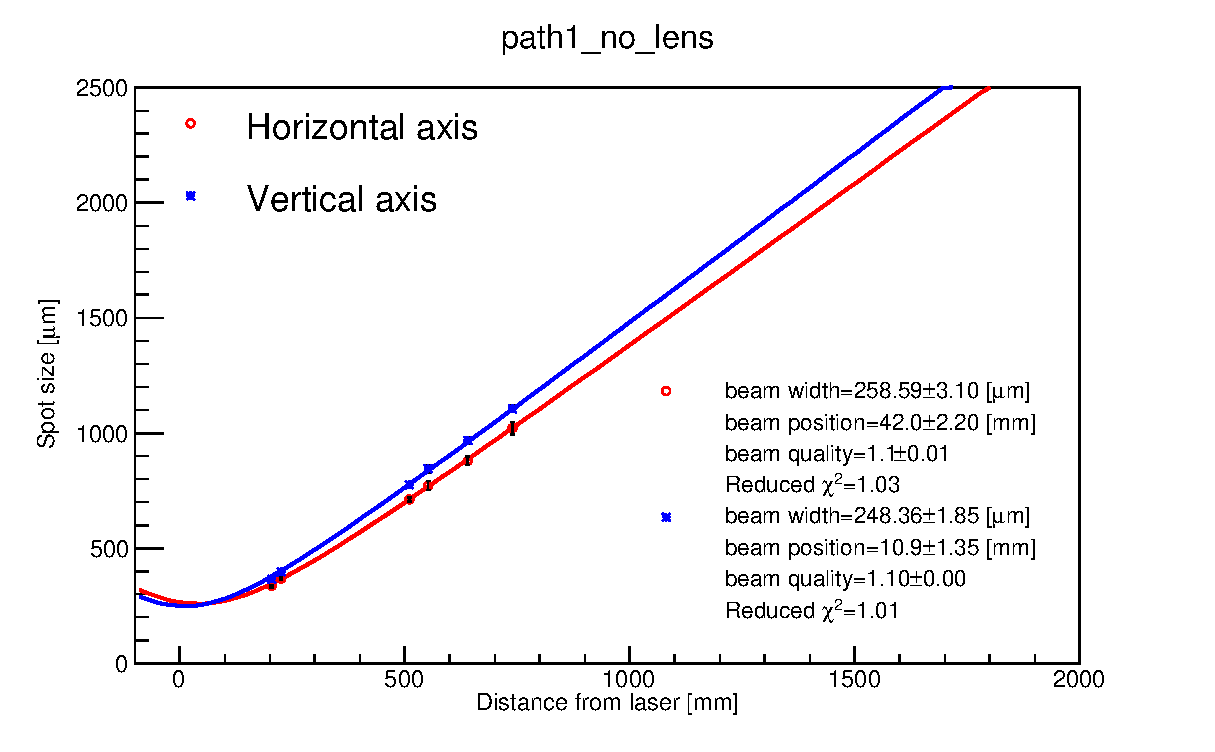
\includegraphics[width=12cm]{path1_no_lens.eps}.

After measuring beam profile, mount the beam splitter, and use power meter to measure the ratio of two paths from the beam splitter. Adjust the angle of incidence of the beam splitter to make the power difference to be less than 1$\%$. The typical value is \underline{\qquad\qquad}. After finishing adjusting beam splitter, install the positive lens for AOM and adjust the height of positive lens to make the laser beam maintain parallel to the optical table. According to the mode matching result, the distance between positive lens and the focus of laser should be 361mm, and the AOM should be mounted at 710mm position. Measure the beam profile around AOM position in two paths and fit the data. The mode matching result and the beam profile around AOM position are shown below:

\begin{center}
	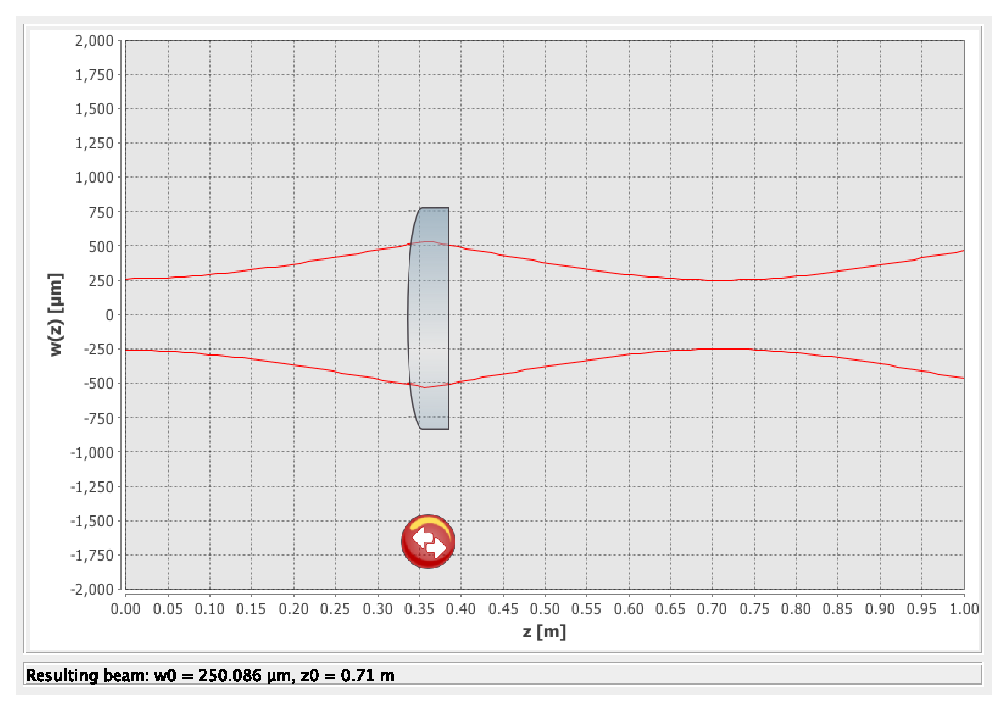
\includegraphics[width=10cm]{modematching_AOM.eps}
	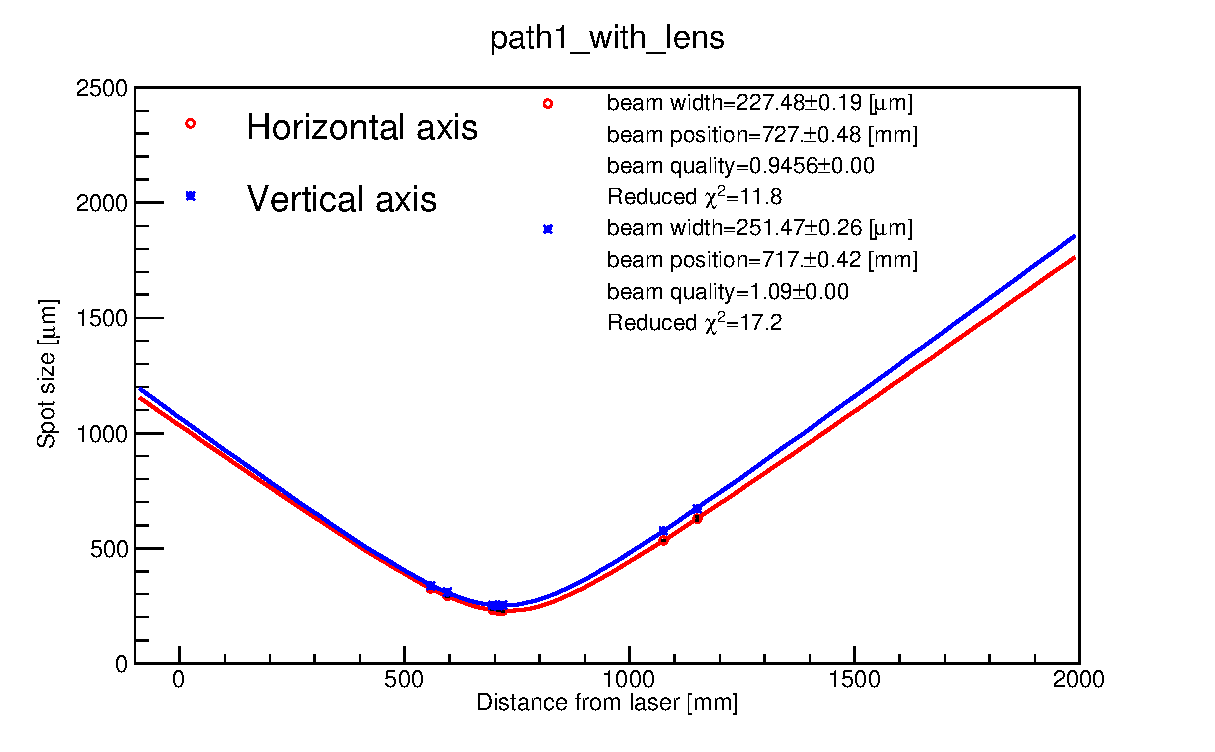
\includegraphics[width=11cm]{path1_with_lens.eps}
	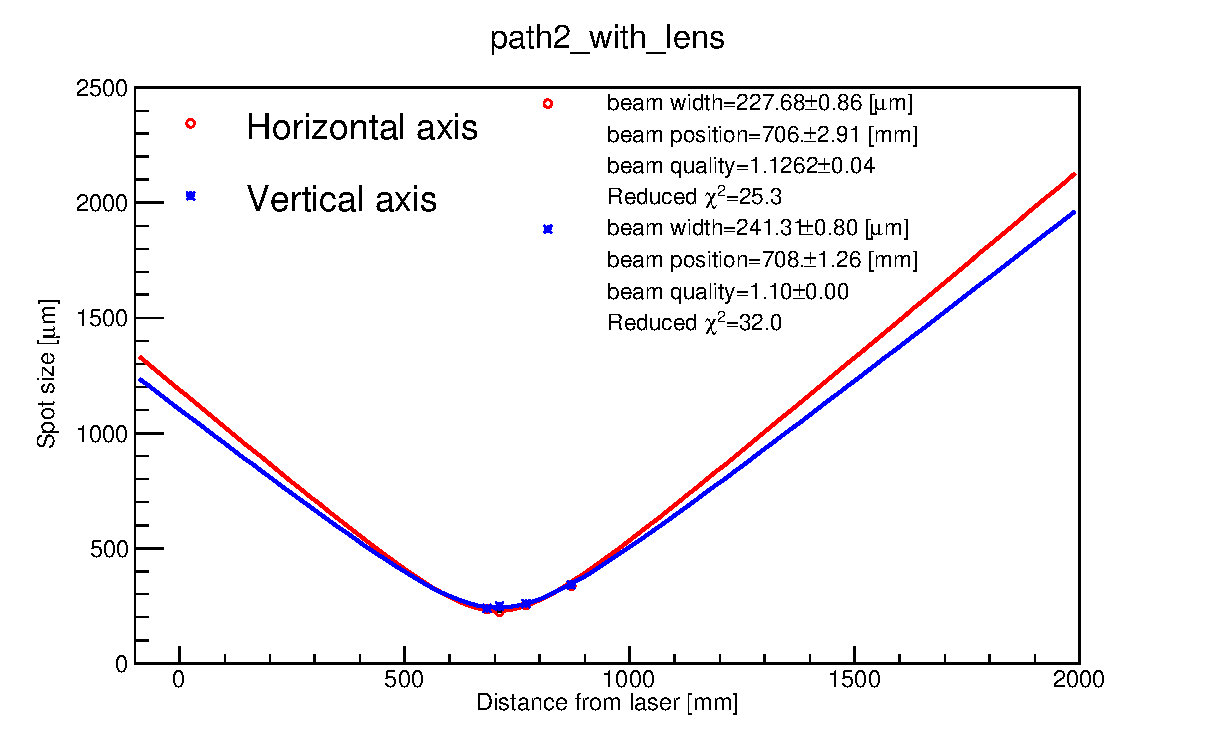
\includegraphics[width=11cm]{path2_with_lens.eps}.
\end{center}



After measuring the beam profile around AOM, install two AOMs at the beam waist for each path. Turn on the laser, send a 1Vdc to AOM by power supply, and adjust the AOM position to enlarge the diffraction efficiency. The largest diffraction efficiency is 93$\%$. Use beam dumper to block the zeroth order beam. Install the polarizer, mirrors, beam sampler, photodetector, integrating sphere. Place a positive lens in front of OFSPD, read the voltage of photodetector by multimeter, and adjust the mirror to enlarge the value. For the mode matching at ETM, place a 1-inch negative lens at 2054mm position, and place a 2-inch positive lens at 2143mm position. The mode matching result is shown in below:

\begin{center}
	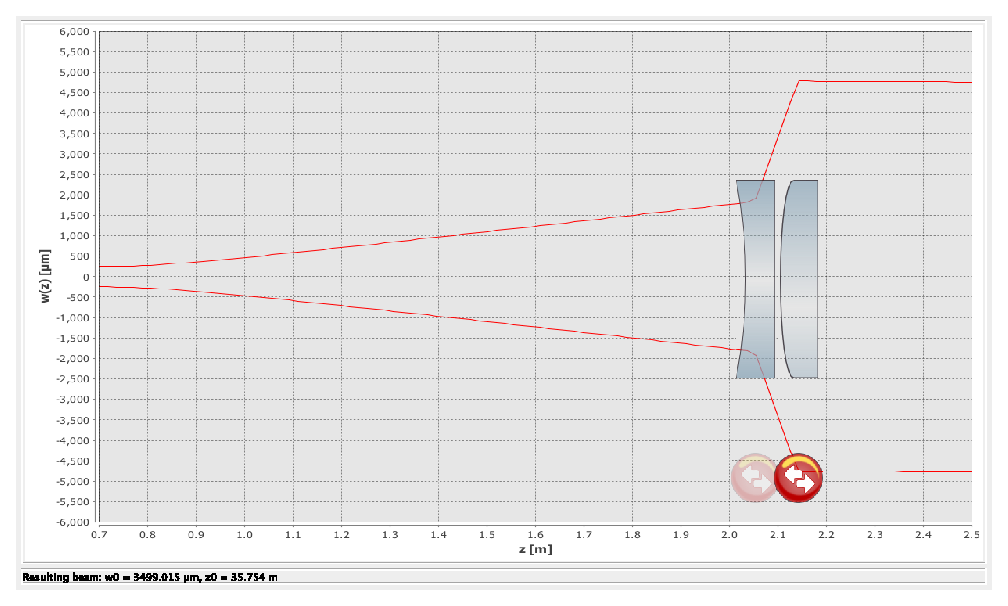
\includegraphics[width=13cm]{modematching_ETM.eps}.
\end{center}


Adjust the height to make the beam inject at the center of the lens to prevent from distortion. Place the final mirror and picomotor, send the beam from transmitter module to receiver module, and reflect the beam into integrating sphere in receiver module.

\section{Transfer function measurement}
\subsection{Open loop measurement}
Turn on the laser and wait for 2 hours until the laser become stable. 
\subsection{Close loop measurement}

\section{Noise measurement}
\subsection{Limitation of Noise}
Basically, we cannot reduce the noise less than sum of electric noise and shot noise when we operate the feedback loop.
\paragraph{Shot noise}
The shot noise can be written by
\begin{equation}
\delta I=\sqrt{2eI},
\end{equation}
where $e$ is elementary charge, I is the current of PD. Then, we can estimate RPN of the shot noise.
\begin{equation}
RPN=\frac{\delta I}{I}=\sqrt{2e/I}.
\end{equation}

			\begin{center}
				\resizebox{13cm}{!}{
					\begin{tabular}{| c | c | c | c | c | c |}
						\hline
						\textbf{Gain of OFSPD1[A/V]} & \textbf{Gain of OFSPD2[A/V]} & \textbf{Offset of OFSPD1 [V]} &\textbf{Offset of OFSPD2 [V]}&\textbf{RPN 1}&\textbf{RPN2}\\ \hline
						 &&&&& \\ \hline
					\end{tabular}
				}
			\end{center}
\paragraph{Electric noise}
\subsection{Relative power noise}
In order to prevent the laser noise from comtaminating the gravitational wave signal, we use 1/10 of KAGRA sensitivity to calculate the Pcal requirement. The following graph is the Pcal requirement:
\begin{center}
	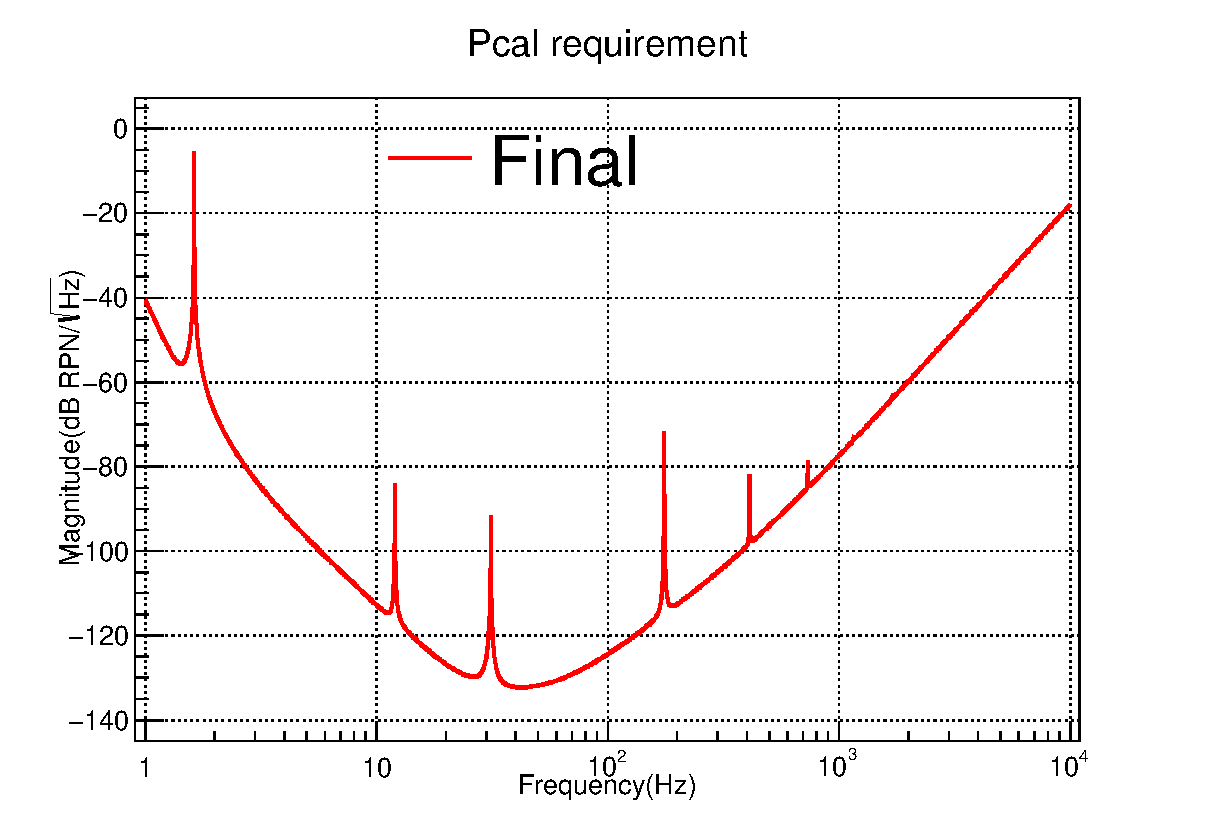
\includegraphics[width=13cm]{pcal_requirement.eps}.
\end{center}

\subsection{Harmonics noise}
\begin{center}
	\resizebox{13cm}{!}{
		\begin{tabular}{| c | c | c |}
			\hline
			\textbf{Injected frequency} & \multicolumn{2}{ c| }{\textbf{7Hz}} \\
			\hline
			 & \textbf{Noise Requirement} & \textbf{Observed value}\\ \hline
			14Hz & -75.1724 & \\ \hline
			21Hz & -83.1094 & \\ \hline
			28Hz & -84.7756 & \\ 
			\hline
		\end{tabular}
	}
\end{center}
\begin{center}
	\resizebox{13cm}{!}{
		\begin{tabular}{| c | c | c |}
			\hline
			\textbf{Injected frequency} & \multicolumn{2}{ c| }{\textbf{35Hz}} \\
			\hline
			& \textbf{Noise Requirement} & \textbf{Observed value}\\ \hline
			70Hz & -58.7316 & \\ \hline
			105Hz & -53.2105 & \\ \hline
			140Hz & -48.3911 & \\ 
			\hline
		\end{tabular}
	}
\end{center}
\begin{center}
	\resizebox{13cm}{!}{
		\begin{tabular}{| c | c | c |}
			\hline
			\textbf{Injected frequency} & \multicolumn{2}{ c| }{\textbf{330Hz}} \\
			\hline
			& \textbf{Noise Requirement} & \textbf{Observed value}\\ \hline
			660Hz & -44.4623 & \\ \hline
			990Hz & -34.5831 & \\ \hline
			1320Hz & -27.3487 & \\ 
			\hline
		\end{tabular}
	}
\end{center}
\begin{center}
	\resizebox{13cm}{!}{
		\begin{tabular}{| c | c | c |}
			\hline
			\textbf{Injected frequency} & \multicolumn{2}{ c| }{\textbf{1KHz}} \\
			\hline
			& \textbf{Noise Requirement} & \textbf{Observed value}\\ \hline
			2KHz & -42.0956 & \\ \hline
			3KHz & -31.6161 & \\ \hline
			4KHz & -24.1504 & \\ 
			\hline
		\end{tabular}
	}
\end{center}
\begin{center}
	\resizebox{13cm}{!}{
		\begin{tabular}{| c | c | c |}
			\hline
			\textbf{Injected frequency} & \multicolumn{2}{ c| }{\textbf{3KHz}} \\
			\hline
			& \textbf{Noise Requirement} & \textbf{Observed value}\\ \hline
			6KHz & -27.1755 & \\ \hline
			9KHz & -16.6197 & \\ 
			\hline
		\end{tabular}
	}
\end{center}

\section{Injection test}
\red{
	I think the time-delay measurement by sine-gaussian signal should be categorized as "Calibration"\\
	Phase reconstruction ?
	\begin{itemize}
		\item Sine-gaussian
		\item CBC NR or EOB waveform
		\item Burst (CCSNe ?)
		\item CW \\	
			I don't understand the practical difficulty of continuous wave injection.
	\end{itemize}
}
\subsection{Hardware Property}
We need to create “inverse actuation filters” in front of injection channel to compensate the effect of $1/f^2$ force-to-length transferfunction, AI filter, overall gain, and OFS transfer function\cite{ligo:inj}.

	\subsubsection{Anti-Imaging Chassis}
\red{Do we need de-whitening chassis to increase effective dynamical range of DGS output?}
	\subsubsection{OFS Low-Pass Filter Transfer Function}



\subsection{File preparation}
\red{How to take care of the inverse transfer function of hardware in each stage.}
	\subsubsection{Compact Binary Coalescence signal}
		\begin{itemize}
			\item BH-BH
			\item BH-NS
			\item NS-NS\\
				\red{the ability of reconstructing post-merger phase}
		\end{itemize}
	\subsubsection{Gravitational Wave Burst Signal}
		\begin{itemize}
			\item CCSNe
		\end{itemize}
	\subsubsection{Continuous Waves Signal}




\subsection{}
\section{Summary}

%----------------------------------------------------------------------------------------

